\documentclass{article}
\usepackage[utf8]{inputenc}
\usepackage{fancyhdr}
\usepackage[margin=2.9cm,twoside]{geometry}
\usepackage[super]{nth}
\usepackage[english]{babel}
\usepackage{csquotes}

\usepackage{hyperref}
\usepackage[backend=biber,style=ieee]{biblatex}
\addbibresource{bibliography.bib}

\pagestyle{fancy}
\fancyhf{}
\fancyhead[LE,RO]{DID - 03 SOR (Hebb \& Stephan)}
\fancyhead[LO,RE]{\leftmark}
\fancyfoot[LE,RO]{\thepage}

% Title Page
\title{Statement of Requirements}
\author{Officer Cadet 27714 Amos Navarre Hebb\\and\\Officer Cadet 27555 Kara Stephan}

\usepackage{graphicx}

\begin{document}
	
\begin{titlepage}
	\begin{center}
		\vspace*{1cm}
		
		\LARGE\textsc{Royal Military College of Canada}\normalsize
		
		\vspace{0.2cm}
		
		\textsc{Department of Electrical and Computer Engineering}
		
		\vspace{1.5cm}
		
		
\includegraphics[width=0.3\textwidth]{rmcLogo.png}
		
		\vspace{1.5cm}
		
		\LARGE{Designing Coatimunde\\}
		
		\vspace{0.2cm}
		
		\normalsize{Computer Optics Analyzing Trajectories In Mostly Unknown, Navigation Denied, Environments}
		
		\vspace{0.1cm}
		
		\normalsize{DID-04 - Preliminary Design}
		
		\vfill
		
		\textbf{Presented by:}\\Amos Navarre \textsc{Hebb} \& Kara \textsc{Stephan}\\
		\vspace{0.8cm}
		\textbf{Presented to:}\\Dr. Sidney \textsc{Givigi} \& Dr. Rachid \textsc{Beguenane}
		\vspace{0.8cm}
		
		\today
		
	\end{center}
\end{titlepage}

% \begin{abstract}
% \end{abstract}

\tableofcontents
\newpage

\section{Introduction}

	\subsection{Document Purpose}
	
	Using Computer Optics for Analyzing Trajectories in Mostly Unknown, Navigation Denied, Environments (\textsc{coatimunde}) is the goal of this project. The purpose of this document is to outline the preliminary design for \textsc{coatimunde}. That is, what the design of the project is, how it will be built, and how this meets the requirements for the project. These requirements have been outlined in the Statement of Requirements. The design of the project thus far will be shown and discussed within the Design Section. This document will then identify the constraints, risks, difficulties that have been faced so far in the project.
	
	\subsection{Background}
	
	Both in the consumer and professional sectors the use of autonomous aerial vehicles is growing quickly. Currently these vehicles rely on skilled pilots to accomplish a very limited set of tasks. Adding obstacle avoidance capabilities to these vehicles and simplifying the task of following targets could allow for these systems to be used in many more situations. This section will give a quick background on obstacle avoidance, unmanned aircraft systems, computer vision, and the platforms we intend to use in this project.
	
		\subsubsection{Obstacle Avoidance}
		
		
		Obstacle avoidance is the task of satisfying a control objective, in this case moving toward a visual target, while subject to non-intersection or non-collision position constraints. The latter constraints are, in this case, to be dynamically created while moving in a reactive manner, instead of being pre-computed.
		
		\subsubsection{Unmanned Aircraft Systems}
		
		Very generally any powered vehicle that uses aerodynamic forces to provide lift without a human operator being carried can be considered an unmanned aerial vehicle. Currently most of these vehicles make up a single component of a larger unmanned aircraft system. 
		
		An Unmanned aircraft system (UAS), or remotely piloted aircraft system (RPAS), is an aircraft without a human pilot on-board, instead controlled from an operator on the ground. Such a system can have varying levels of autonomy, something as simple as a model aircraft could be considered a UAS without any automation capabilities. Detecting, recognizing, identifying, and tracking targets of interest in complex environments and integrate with the systems required to process and fuse the collected information into actionable intelligence while operating in a low-to-medium threat environment is the current goal of the RPAS project by the Royal Canadian Air Force (RCAF) \cite{RPAS}. 
		
		Flying a UAS requires a secure link to the operator off-board. Maintaining this link, particularly while flying close to the ground where more opportunities for interference are introduced is difficult. This difficulty is compounded in environments where potentially hostile actors may be attempting to jam communications. This necessitates a level of automation on-board capable of maintaining flight while denied navigation information.
		
		There are many different types of approaches for this problem, but most involve some form of identifying targets in real time and reacting as they become visible to the aircraft. This has proven successful on a flying robot traveling at high speeds \cite{barry2015pushbroom}. This system successfully combined trajectory libraries and a state machine to avoid obstacles using very little computational power even at very high speeds \cite{barry2018high}. Another solution to obstacle avoidance on flying robots was the creation of NanoMap \cite{2018nanomap}. This allows for 3D data to be processed at a much faster rate allowing for higher speeds of the robot \cite{2018nanomap}.
		
		\subsubsection{Computer Vision}
		
		Currently there are many different ways that computers can make high-level decisions based on digital image information. There are many methods to acquire, process, and analyze data from the real world using a camera. While this is a very broad field, we intend to focus especially on the aspects around motion estimation and object recognition. Both will be working with a video stream taken from a camera. 
		
		Motion estimation can be accomplished using direct methods which compare whole fields of pixels to each other over successive frames, compared to indirect methods which look for specific features. The information resulting from motion estimation streams can be used to both compensate for motion while analyzing other aspects of an image, and update a state machine.
		
		Object recognition in our project will be accomplishing two tasks. Identifying a marker or target which will require more involved object recognition calculations, and very simple techniques, such as edge detection, to identify obstacles that exist in the path of the robot.
		
		\subsubsection{OpenCV}
		
		The Open Source Computer Vision Library (OpenCV) of programming functions is a cross-platform and free for use collection of functions primarily aimed at real-time computer vision\cite{opencv}. Most well documented techniques to accomplish all of the computer vision goals of our project have already been created and refined in OpenCV. For this reason we will be leaning heavily on OpenCV functions.
		
		\subsubsection{Gazebo}
		
		Gazebo is a robot simulator that allows for creation of a realistic environment which includes both obstacles and markers similar to those being used in the lab. It will then be used to rapidly test algorithms.
		
		\subsubsection{Robot Operating System}
		
		The Robot Operating System (ROS) is a distributed message system that allows for various sensors and processors to work together to control a robot. It is open source and has been integrated already with OpenCV and Gazebo. There are many additional tools for detecting obstacles, mapping the environment, planning paths, and much more. It is also a robust messaging system that has been proven to be capable of real-time processes.
		
		\subsubsection{TurtleBot}
		
		The TurtleBot is a robot kit with open-source design and software. A TurtleBot is a robot built to the specification for TurtleBot Compatible Platforms\cite{wise_foote_2011}. In our case this is a Kobuki Base, an Acer Netbook running Ubuntu with ROS packages added, an X-Box Kinect, and some mounting plates. 
		
		The resulting robot looks like a disk supporting some circular shelves with a small laptop and a camera on the shelves. The base disk is 35.4cm in diameter, the topmost shelf is 42cm from the ground. The robot has a maximum speed of 0.65m/s. 
		
		\subsubsection{AscTec Pelican}
		
		The Ascending Technologies Pelican is a 65.1cm by 65.1cm quad-rotor  designed for research purposes\cite{asctec}. It includes a camera, a high level and low level processor set up for computer vision and SLAM research. It is also capable of interfacing easily with other controllers and can carry up to a kilogram of additional gear.
		
\section{Design Section}

	Computer Optics Analyzing Trajectories In Mostly Unknown, Navigation Denied, Environments or coatimunde is the name of this project. 
Computer optics is used as the robot will be using a camera to identify any important surroundings such as, a target or an obstacle. 
Analyzing trajectories is a term that refers to the robot completing movements to go towards the target. To do path planning the project will implement potential fields. Potential fields work through having vectors that point to object and assigning as positive or negative. The positive vectors attracts the robot towards the target and the negative makes obstacles repulsive to the robot \cite{hwang1992potential}. This algorithm was selected to do path planning as the robot won't have to build a map of the environment to create path to the target \cite{bortoff2000path}. Potential fields allows for the robot to change its path along the way if it discovers new obstacles. The project will also implement a state machine to update the position of the vectors when the robot is moving. This ensures that the robot always knows where the target and identified obstacles are when its own position changes. Navigation denied means that the robot will not have access to a GPS to locate itself, it must search its unknown environment to identify targets and obstacles. An unknown environment can be defined as an environment in which the robot has no prior knowledge to its surroundings and must identify objects in this environment itself through computer vision. This once again is the reason that the project will be using potential fields to plan the path to the target. 
	The aim of this project is to build an air robot that is able to identify a target and move toward it, avoiding any obstacles that are in the way. Tracking targets of interest in complex environments with a flying robot is the ultimate goal of this project. To accomplish this goal we will be using a TurtleBot and then a UAV with only one camera to identify targets and obstacles. 


	\subsection{Block Diagram}
	The block diagram that is shown in Figure \ref{fig:blockdiagram} contains the outline of the \textsc{coatimunde} project. It is a very high level overview and does not contain references to most of the hardware in use for two reasons. The first reason is that the actual robot and laptop being used are relatively arbitrary as long as the software included is present on both. ROS being used also includes many nodes which are not included, only the ones that are most important to our project, will have to be specifically added to ROS, or will have to be custom created are included on our system block diagram.
	
	The laptop contains the initialization, target selection, and RViz. The laptop also takes the user input when necessary and processes it appropriately.  The robot will do all the target identification, obstacle avoidance, and movement decisions autonomously. This means it will take input from the camera into a video processing node and then create a corresponding ROS message to be sent to the other systems on the robot. These messages are created and used throughout the different systems on the robot. The model of the robot's environment will be found subscribing to messages from the obstacle finder node, target finder node, and the state estimate node. This model then creates a message to pass to the route planning node which tells the movement node how to update its position and speed. 

	\begin{figure}
		\centering
		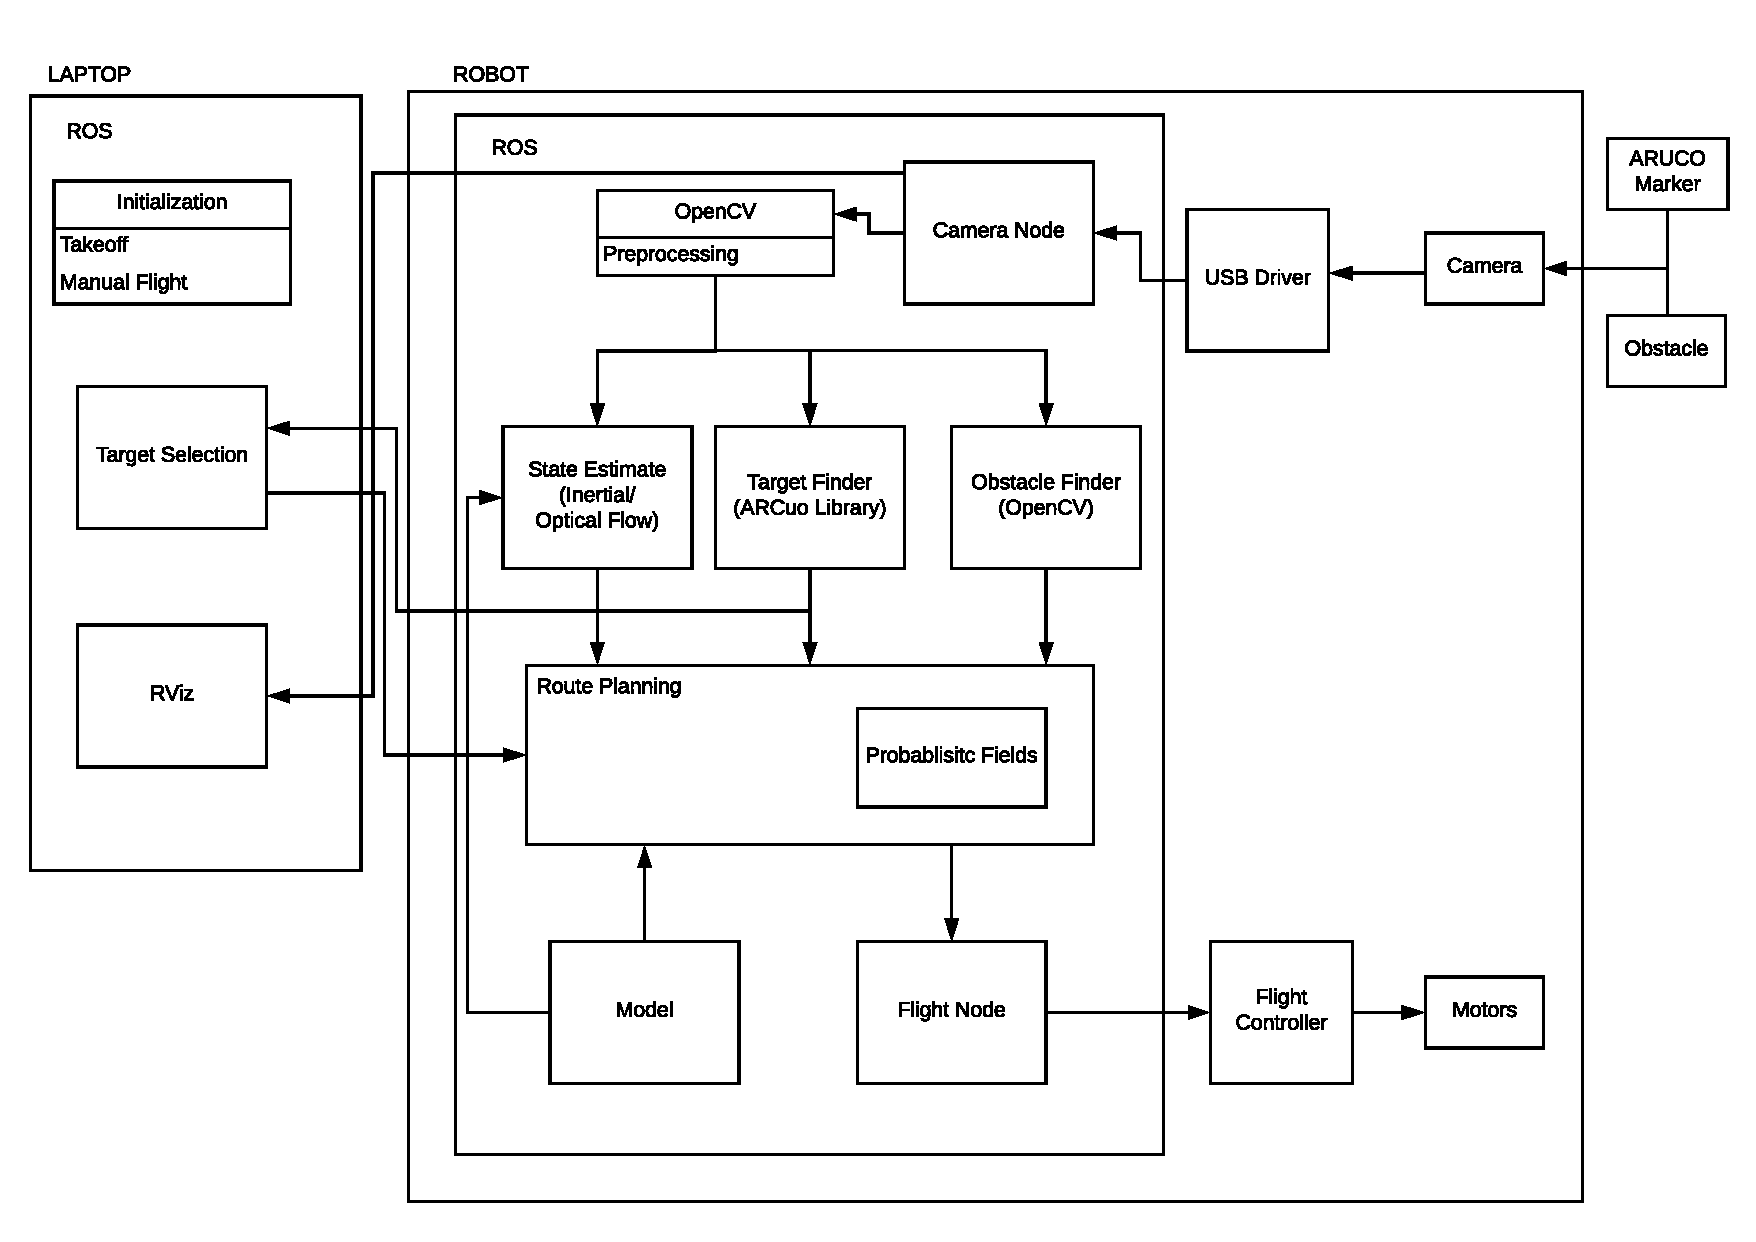
\includegraphics[width=0.9\linewidth]{BlockDiagram}
		\caption{Project Schedule Diagram}
		\label{fig:blockdiagram}
	\end{figure}

	\subsection{Node Diagram}

	\begin{figure}
		\centering
		\includegraphics[width=0.9\linewidth]{NodeDiagram}
		\caption{Project Node Diagram}
		\label{fig:nodediagram}
	\end{figure}

Through Figure {fig:nodediagram} it can been shown what nodes will be created for this project. All nodes in the project will be written in python and then built in ROS to be implemented on the robot. The diagram displays what node will subscribe to the other nodes, such as the simple target finder node will subscribe to the video processor node to get messages about the target's potential location. Both the TurtleBot and the Flying Robot have two movement nodes, this is to first build a simple movement node on the platform for testing purposes. Then the proper and final movement node will be made and implemented on the respective robot. 
	
	\subsection{Mathematical Modeling}
	
		\subsubsection{Flying Robot}
	
	Given that a quad-copter has six degrees of freedom, modeling them is a very difficult task. The AscTec Pelican already has many existing models indented for use with ROS. There is also a large collection of hardware agnostic tools for operating a quad-copters.
	
		\subsubsection{Robot in 3D Space}
	
	The robot itself will need to remember where it is located in its environment. Remembering where targets are located relative to the robot is necessary, and presumably remembering the locations of obstacles will be used as well. Using quaternion vectors relative to the robot will allow for simple transformations on these vectors while using very little computational power. ROS contains methods and messages to easily communicate, convert, and apply transformations to quaternions.
	
		\subsubsection{Pose Estimation}
	
	Initially feedback from inertial sensors will be used for pose estimation, but ideally a version of Optical Flow would be used to estimate the position of the robot in 3D space. There are some libraries in OpenCV that have addressed generalized pose estimation in 6 degrees of freedom, but it requires a significant amount of computational power, a higher frame rate than our goal of 10Hz to be used for real time performance, and hundreds of visual odometry measurements must be made in every frame requiring a visually busy background.

	\subsection{Interfacing}
	
	The interfacing of almost all sensors with the on-board computer will be done over USB. Between different nodes on the same computer, and any computers off-board the robot, will be done exclusively with ROS messages sent over either internal loops or Wi-Fi.

	\subsection{Verification and Validation TODO}
-Gazebo
-Camera tests
-Actually using the robot

Verification and validation of the project's nodes will be done prior to implementation in the Gazebo simulation environment. Gazebo scheduled timelines can be seen in Figure {fig:scedulediagram}. 


\section{Equipment}

	\subsection{Equipment Table}
	
	%But in a big array here


\section{Schedule}

\begin{table}[]
	\begin{tabular}{|l|r|l|l|}
		\hline
		\multicolumn{1}{|c|}{\textbf{Task Name}}            & \multicolumn{1}{c|}{\textbf{Duration}} & \multicolumn{1}{c|}{\textbf{Start}} & \multicolumn{1}{c|}{\textbf{Finish}} \\ \hline
		\textbf{Coatimunde}              		    & \textbf{144 days} & \textbf{Tue 09/10/18} & \textbf{Sun 28/04/19} \\ \hline
		\textbf{- Turtlebot}                                & \textbf{97 days}  & \textbf{Tue 09/10/18} & \textbf{Wed 20/02/19} \\ \hline
		-- Create a Basic Movement Node                     & 12 days           & Tue 09/10/18          & Wed 24/10/18          \\ \hline
		-- Subscribe to the Camera                          & 8 days            & Wed 24/10/18          & Fri 02/11/18          \\ \hline
		\textbf{-- Camera and Video}                        & \textbf{19 days}  & \textbf{Tue 30/10/18} & \textbf{Fri 23/11/18} \\ \hline
		--- OpenCV able to process Video Stream 	    & 9 days            & Tue 30/10/18          & Fri 09/11/18          \\ \hline
		--- Able to detect a Target                         & 12 days           & Tue 08/11/18          & Fri 23/11/18          \\ \hline
		\textbf{-- Movement}                                & \textbf{67 days}  & \textbf{Tue 20/11/18} & \textbf{Wed 20/02/19} \\ \hline
		--- Move towards Target                             & 9 days            & Tue 20/11/18          & Fri 30/11/18          \\ \hline
		--- Avoid Obstacles and Move Towards Target         & 31 days           & Thu 29/11/18          & Thu 10/01/19          \\ \hline
		--- Avoid Obstacles with Memory 		    & 32 days           & Tue 08/01/19          & Wed 20/02/19          \\ \hline
		\textbf{- UAV}                                      & \textbf{53 days}  & \textbf{Wed 13/02/19} & \textbf{Sun 28/04/19} \\ \hline
		-- Port to UAV                                      & 53 days           & Wed 13/02/19          & Sun 28/04/19          \\ \hline
		\textbf{-Data Item Deliverables (DID)}		    & \textbf{148 days} & \textbf{Thu 01/11/18} & \textbf{Thu 28/03/19} \\ \hline
		-- DID-4 Preliminary Design Specification	    & 22 days		& Thu 01/11/18		& Thu 22/11/18		\\ \hline
		-- DID-5 Design Review Presentation		    & 15 days		& Thu 15/11/18		& Thu 29/11/18		\\ \hline
		-- DID-6 Schedule Update			    & 56 days		& Fri 30/11/18		& Thu 17/01/19		\\ \hline
		-- DID-7 Detailed Design Document		    & 63 days		& Fri 18/01/19		& Thu 21/03/19		\\ \hline
		-- DID-8 Final Project Presentation		    & 148 days		& Thu 01/11/18		& Thu 28/03/19		\\ \hline

	\end{tabular}
	\caption{Project Schedule Table}
	\label{table:projectscheduletable}
\end{table}

\begin{figure}
	\centering
	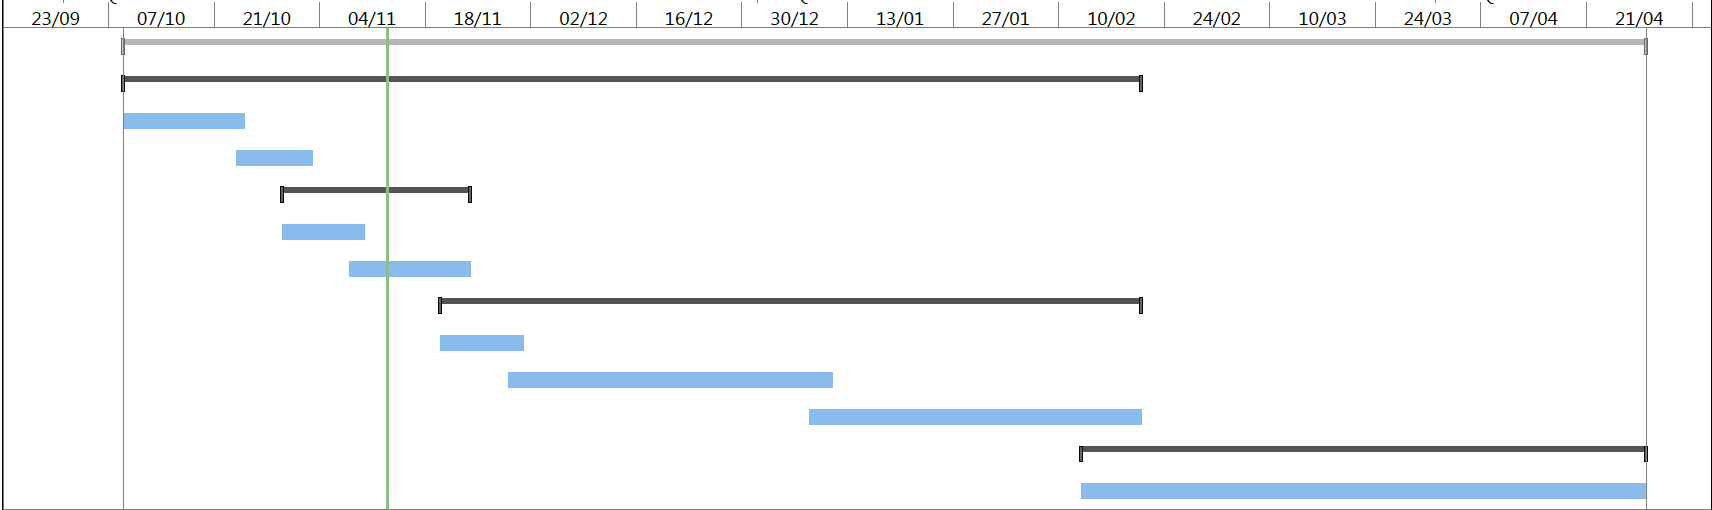
\includegraphics[width=\linewidth]{ScheduleDiagram}
	\caption{Project Schedule Diagram}
	\label{fig:schedulediagram}
\end{figure}

The created schedule for the project is shown above. This outlines the major milestones for the project, such as Data Item Deliverables and deadlines for completing different functionalities for the project. Porting to the UAV is listed as one task as we aren't sure what problems will arise until we attempt to port the project.  

\section{Unresolved Issues and Risks}

	\subsection{Limited Space}
	The scope of the project is limited due to only being able to test indoors. Ideally the UAV would be operating at a high speed and identifying an arbitrary target in an unpredictable environment. In our case though the testing must be completed within the confines of a relatively small robotics laboratory. Smaller obstacles will be used indoors simply due to space constraints. Lower speeds will be used as well, again due to the lack of space. 

	\subsection{Identifying Markers}
	
	The markers we intend to use, at least initially, are intended for use in Augmented Reality purposes. Tests of these shapes show that they are capable of being identified at many angles, but the reliability with which they can be identified decreases quickly as the viewing angle changes. 
	
	There is potential that markers which are reliably identified at low speeds and in simulation may not be detectable on a flying vehicle moving faster.
	
		\subsubsection{Likelihood}
 
		Both the TurtleBot and Flying Robot shall be traveling at lower speeds, therefore the likelihood of this risk is low.
		
		\subsubsection{Impact}
		
		High impact, the primary task that our robot must accomplish is moving toward a visual target. If the robot is not able to reliably identify a marker then there will be no way to verify its capability.
		
		\subsubsection{Process Solution}
		
		Alternatives to the ArUco markers can be tested, or if these prove truly unreliable then coloured areas or illuminated targets could be incorporated. These are less desirable as ideally the robot would be able to fly toward an arbitrary target.
		
	\subsection{Computer Hardware Limitations}
	
	Image processing, especially quickly and with multiple goals, is computationally expensive. While this should not be an issue on a ground vehicle moving at slower speeds, it may become more of an issue on a Flying Robot if it operates at higher speeds and is incapable of carrying as much on-board computational capability.
	
		\subsubsection{Likelihood}

		High likelihood due to the amount of computational power required to do image processing. 
		
		\subsubsection{Impact}
		
		Medium impact, presumably we would still be able to prove our systems on the ground robot which is capable of carrying as much processing power as needed. It may also only be a limitation at higher speeds or may impose limits on what the Flying Robot is capable of identifying and tracking. 
		
		\subsubsection{Process Solution}
		
		Testing many algorithms and working to streamline the algorithm used, especially for the Flying Robot, as well as selecting hardware that is complimentary to the kind of loads created by running such an algorithm can mitigate these risks. Using an FPGA could aid with this problem.
	
	\subsection{Flight Control System Inaccuracy}
	
	Many UAV's are not able to execute arbitrary movements with high accuracy. Verifying that the drone is actually executing instructions may be difficult. 
	
		\subsubsection{Likelihood}
		
		Medium likelihood, depending on how well developed the libraries for our particular drone these issues may have all been sufficiently worked out for the purposes of this project.
		
		\subsubsection{Impact}
		
		Low impact, we could still observe the Flying Robot making decisions even if it is unable to execute the instructions given properly.
		
		\subsubsection{Process Solution}
		
		Using smaller number of obstacles and moving at a slow enough speed should ensure that the robot never needs to execute extreme moves. These more extreme moves are where inaccuracies in control models will exposes themselves the most. 



\section{Conclusion}
The preliminary design has been shown for the Flying Robot obstacle avoidance system. Background and requirement defining activities have been given to lay the groundwork and a basic understand of the current research in this domain. This document will be used and referenced for the rest of the design and building processes for the project. The design laid out in this document will also be used in the the Preliminary Design Review and Detailed Design Document. 



\printbibliography

%\end{multicols}
\end{document}    

